% 2003 年全国旧课程理科第 15 题：行政区域着色图
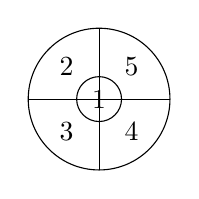
\begin{tikzpicture}[scale=0.75]
  \draw (0,0) circle (1.2);
  \draw (0,-1.2)--(0,1.2) (-1.2,0)--(1.2,0);
  \draw (0,0) circle (0.38);
  \node at (0,0) {1};
  \node at (-0.55,0.55) {2};
  \node at (0.55,0.55) {5};
  \node at (-0.55,-0.55) {3};
  \node at (0.55,-0.55) {4};
\end{tikzpicture}
